\documentclass[10pt,aspectratio=169]{beamer}

\usepackage[english]{babel}
\usepackage[utf8]{inputenc}
\usepackage{graphicx}
\usepackage{amsfonts,amsmath,amssymb}
\usepackage{epstopdf}
\usepackage{soul}
\usepackage{float}
\usepackage[font=small]{caption, subcaption}
\usepackage{etoolbox}

\usetheme{Clean}
\useinnertheme[shadow=true]{rounded}
\usetikzlibrary{calc}

%% New Block Colors !!
\setbeamercolor{block title example}{use=example text,fg=example text.fg,bg=example text.fg!20!bg}
\setbeamercolor{block body example}{parent=normal text,use=block title example,bg=block title example.bg!50!bg}
\setbeamercolor{block title alerted}{use=alerted text,fg=alerted text.fg,bg=alerted text.fg!20!bg}
\setbeamercolor{block body alerted}{parent=normal text,use=block title alerted,bg=block title alerted.bg!50!bg}
\setbeamercolor{block title}{use=structure,fg=structure.fg,bg=structure.fg!20!bg}
\setbeamercolor{block body}{parent=normal text,use=block title,bg=block title.bg!50!bg}

\BeforeBeginEnvironment{problem}{
    \setbeamercolor{block title}{fg=red!50!black,bg=red!30!white}
    \setbeamercolor{block body}{fg=black, bg=red!10!white}
}
\AfterEndEnvironment{problem}{
 \setbeamercolor{block title}{use=structure,fg=structure.fg,bg=structure.fg!20!bg}
 \setbeamercolor{block body}{parent=normal text,use=block title,bg=block title.bg!50!bg, fg=black}
}

\title[Motion Planning \& Control]
		{On The Motion Planning \& Control of Nonlinear Robotic Systems}

\author[L. Gentilini]
			{Lorenzo Gentilini \\
				{\textit{\href{mailto:lorenzo.gentilini6@unibo.it}{lorenzo.gentilini6@unibo.it}}}
			}

\date{June 15, 2023}

\newcommand*\titleSubsec{Outline}
\newcommand*\titleTOC{Outline}

\beamertemplatenavigationsymbolsempty
\newtheorem{assumption}[theorem]{Assumption}

\begin{document}
\footnotesize

% Title Slide %%%%%%%%%%%%%%%%%%%%%%%%%
\begin{frame}[plain,noframenumbering,t]
	\centering

	\vspace{1.5cm}
	\textcolor{blue@O4S}{\Large \inserttitle}

	\vspace{1cm}
	\begin{columns}[t]
		\column{0.2\linewidth}
		% Dummy Column

		\column{0.2\linewidth}
		\centering
		\textit{Ph.D. Candidate} \\ \vspace{0,1cm} {\normalsize Lorenzo Gentilini}

		\column{0.2\linewidth}
		\centering
		\textit{Ph.D. Supervisor} \\ \vspace{0,1cm} {\normalsize Lorenzo Marconi}

		\column{0.2\linewidth}
		% Dummy Column
	\end{columns}

	\vspace{1.5cm}
	\textit{Ph.D. in Biomedical, Electrical, and System Engineering}

	\vspace{0.3cm}
	\textcolor{emph@O4S}{
		\textit{
			Dept.~of Electrical, Electronic and Information Engineering, \\
			Alma Mater Studiorum University of Bologna, Bologna, Italy \\
			(e-mails: \{lorenzo.gentilini6, lorenzo.marconi\}@unibo.it).
		}
	}
\end{frame}

% Slide 1 %%%%%%%%%%%%%%%%%%%%%%%%%
\begin{frame}[t]{What If Robotics and System Theory Met By Mistake?}
	\vfill
	\textcolor{emph@O4S}{\textit{Intuition:}} \\
	As long as robotics and system theory develops independently we shall never reach cutting-edge solutions.

	\vspace{0.2cm}
	\textcolor{emph@O4S}{\textit{Objectives:}} \\
	\begin{itemize}
		\item[1] Join the two fields of robotics and control theory.
		\item[2] Let both of them borrow tools from its counterpart.
		\item[3] Improve domain-specific solutions.
	\end{itemize}

	\vspace{0.2cm}
	\textcolor{emph@O4S}{\textit{Methods:}} \\
	\begin{itemize}
		\item[1] Identify a possible common point.
		\item[2] Develop both robotics and system solutions around the identified link.
		\item[3] Approach a specific-domain problem borrowing tool from both fields.
	\end{itemize}

	\vfill
	\begin{columns}
		\column{0.3\linewidth}
		\begin{block}{\centering Robotic View}
			\centering
			Development of a fully autonomous aerial vehicle for indoor flight.
		\end{block}

		\column{0.3\linewidth}
		\begin{alertblock}{\centering Common Joint Link}
			\centering
			Gaussian process regression, a new paradigm to unsupervised learning.
		\end{alertblock}

		\column{0.3\linewidth}
		\begin{exampleblock}{\centering System View}
			\centering
			Development of nonlinear control techniques, focusing on the field of output regulation.
		\end{exampleblock}
	\end{columns}
\end{frame}

% Slide 2 %%%%%%%%%%%%%%%%%%%%%%%%%
\begin{frame}[t]{The Leonardo Drone Contest}  
	\begin{columns}[t]
		% Column 1
		\column{0.5\linewidth}
		\begin{exampleblock}{Main Goal}
			Implement, deploy, and test autonomous navigation algorithms for drones in applications of GPS-denied indoor flight.
		\end{exampleblock}		

		\vspace{0.2cm}
		\textcolor{emph@O4S}{\textit{Developed Solutions:}} \\
		\begin{itemize}
			\item[1] Environment mapping and localisation.
			\item[2] Environment exploration and patrolling.
			\item[3] Trajectory planning and optimisation.
			\item[4] Trajectory replanning for obstacle avoidance.
			\item[5] Precise landing on spots. 
			\item[6] Buildings inspection.
			\item[7] Object tracking.
			\item[8] Text detection and recognition.
		\end{itemize}

		% Column 2
		\column{0.5\linewidth}
		\begin{figure}[!t]
			\centering
			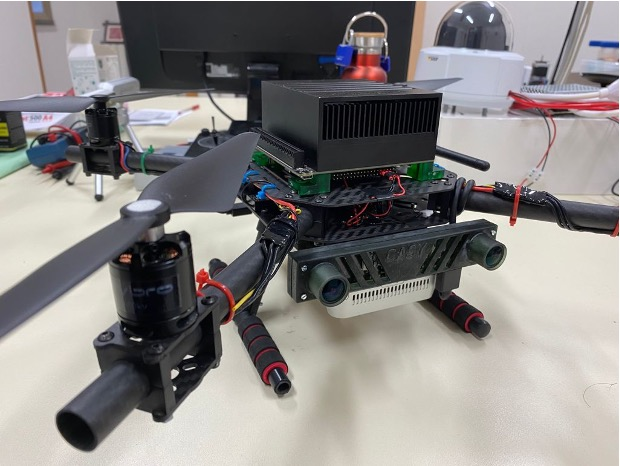
\includegraphics[width=0.64\textwidth]{../Figs/Chapter1/drone.pdf}
			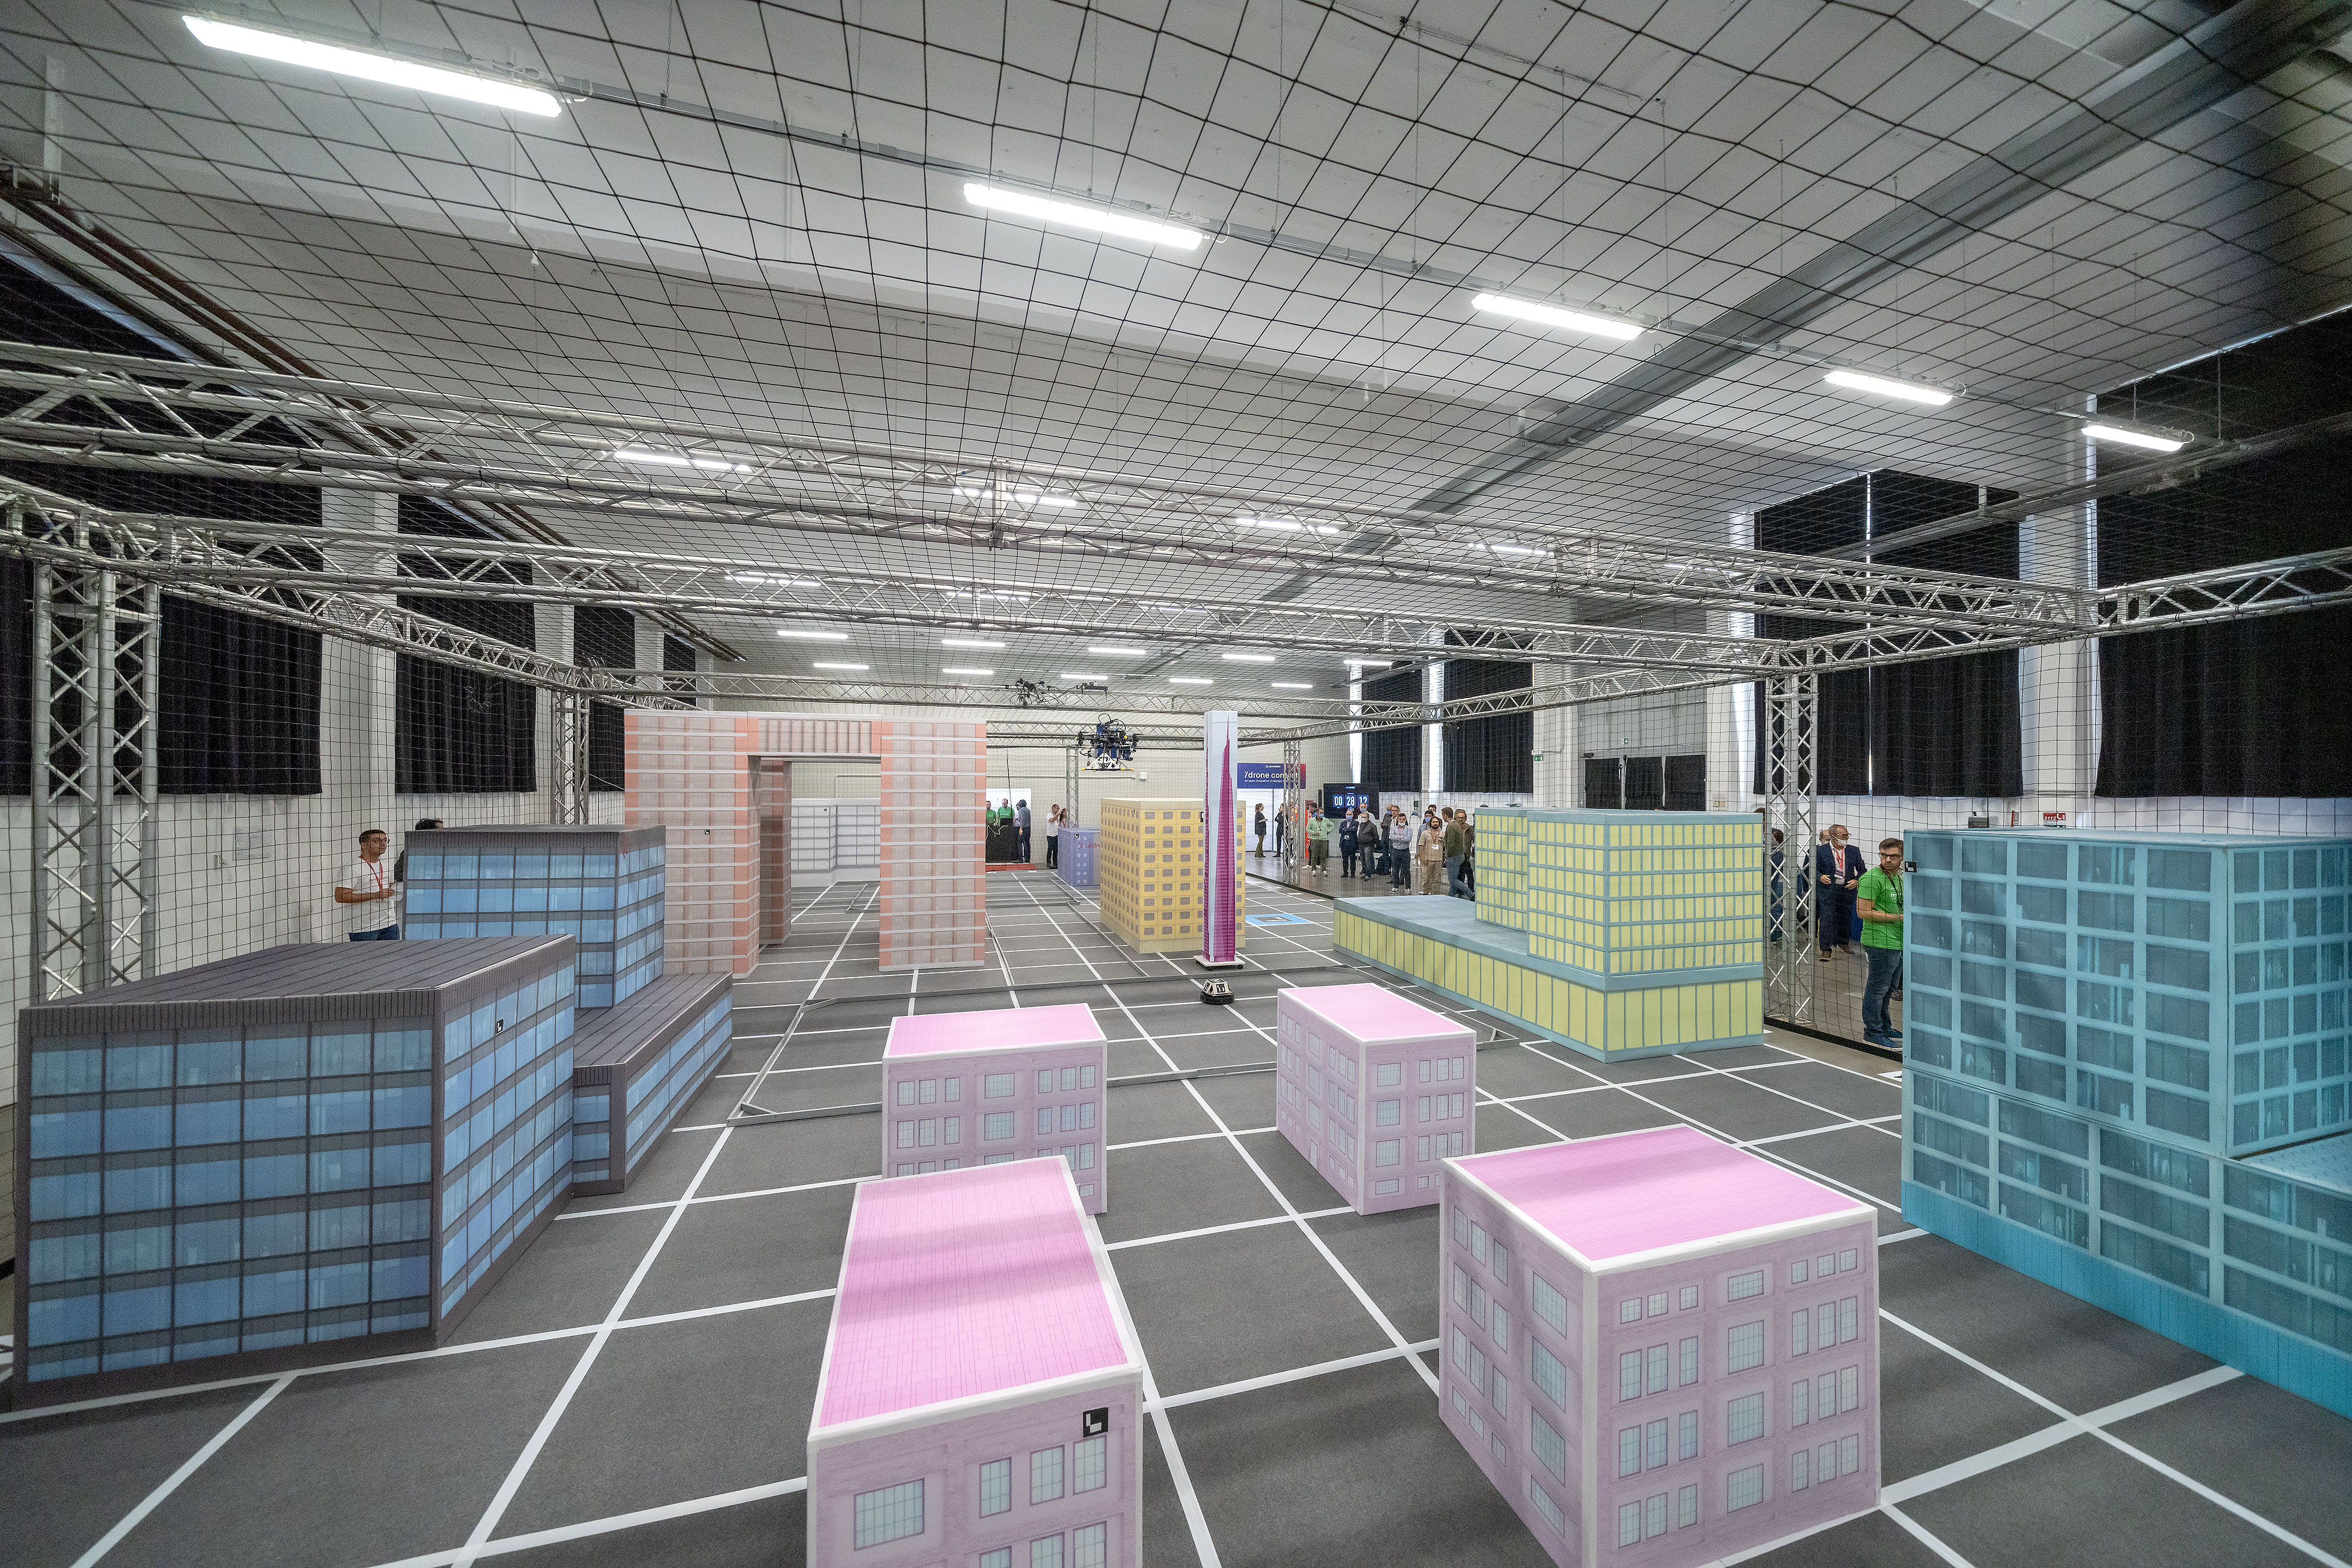
\includegraphics[width=0.6\textwidth]{../Figs/Chapter1/leonardo_map.jpg}
		\end{figure}
	\end{columns} 
\end{frame}

% Slide 3 %%%%%%%%%%%%%%%%%%%%%%%%%
\begin{frame}[t]{Common Link: Gaussian Process Inference}  
	
\end{frame}

% Slide 4 %%%%%%%%%%%%%%%%%%%%%%%%%
\begin{frame}[t]{Gaussian Process Inference}  
	
\end{frame}

% Slide 5 %%%%%%%%%%%%%%%%%%%%%%%%%
\begin{frame}[t]{Autonomous Environment Exploration}
	
\end{frame}

% Slide 6 %%%%%%%%%%%%%%%%%%%%%%%%%
\begin{frame}[t]{Autonomous Environment Exploration}
	
\end{frame}

% Slide 7 %%%%%%%%%%%%%%%%%%%%%%%%%
\begin{frame}[t]{Autonomous Areas Patrolling}
	
\end{frame}

% Slide 8 %%%%%%%%%%%%%%%%%%%%%%%%%
\begin{frame}[t]{Autonomous Areas Patrolling}
	
\end{frame}

% Slide 9 %%%%%%%%%%%%%%%%%%%%%%%%%
\begin{frame}[t]{Data-Driven Control Barrier Functions}  
	
\end{frame}

% Slide 10 %%%%%%%%%%%%%%%%%%%%%%%%%
\begin{frame}[t]{Data-Driven Control Barrier Functions}  
	
\end{frame}

% Slide 11 %%%%%%%%%%%%%%%%%%%%%%%%%
\begin{frame}[t]{Adaptive Nonlinear Output regulation}  
	
\end{frame}

% Slide 12 %%%%%%%%%%%%%%%%%%%%%%%%%
\begin{frame}[t]{Adaptive Nonlinear Output regulation}  

\end{frame}
\end{document}
